\documentclass[14pt,a4paper,oneside]{article}

\usepackage[utf8]{inputenc}   


\usepackage{amsmath,amsthm,amssymb,appendix,bm,mathrsfs,ctex,geometry,tcolorbox,fancyhdr,tikz,esint,appendix}


%% GB/T 7714 宏包 ---- 引文格式
\usepackage[sort&compress]{gbt7714}
\bibliographystyle{gbt7714-numerical}



% \numberwithin{equation}{section}             %%%%%% 公式编号




\geometry{left=1.7cm, right=1.7cm, top=2.54cm, bottom=2.54cm}    %%%%% 页面尺寸
\linespread{1.5}                             %%%%% 行距1.5倍
\pagestyle{fancy}



%%    设置页眉页脚
\fancyhf{}
\renewcommand{\headrulewidth}{0.15mm}
\fancyhead[C]{文献阅读报告}                   %%%%%% 页眉
\fancyfoot[C]{\thepage}                      %%%%%% 页脚 页码
\setlength{\headheight}{15pt}


%%   设置各种链接颜色为黑色
\usepackage[colorlinks,
            linkcolor=black,
            anchorcolor=black,
            citecolor=black,
            urlcolor=blue
            ]{hyperref}



%%   例子编号
\newcounter{example}
\counterwithin{example}{subsection}
\newcommand{\examplename}{Example}
\newcommand{\exampleTitle}[1]{%
\textbf{\refstepcounter{example}\examplename\theexample:#1}\par}


%%  插入图片配置
\usepackage{graphicx,subfigure}
\usepackage[]{caption2} %新增调用的宏包
% \numberwithin{figure}{section}               %%%%%% 图片编号按节

\graphicspath{ {./Figure/} }            %%%%% 设置图片文件所在目录
\DeclareGraphicsExtensions{.pdf,.svg,.jpeg,.png,.jpg}     %%%%% 支持图片格式


%%    支持tikz作图
\usepackage{tikz}
\usetikzlibrary{backgrounds,arrows}


\usepackage{pgfplots}
\pgfplotsset{compat=1.15}
\usepackage{mathrsfs}


\title{\textbf{文献阅读报告 13\\Millijoule few-cycle pulses from staged compression for strong and high field science}\cite{stanfieldMillijouleFewcyclePulses2021}}                           %%%%% 标题
\author{骆禹天}                                           %%%%% 作者
\date{2024/**/**}                                        %%%%%% 日期

%%   定义一些数学格式
\newtheorem{theorem}{定理}[]
\newtheorem{definition}[theorem]{定义}
\newtheorem{lemma}[theorem]{引理}
\newtheorem{corollary}[theorem]{推论}
\newtheorem{example}[theorem]{例}
\newtheorem{proposition}[theorem]{命题}
\renewcommand{\abstractname}{\Large\textbf{摘要}}




%------------------------- 开始文档  -------------------------%



\begin{document}

\pagenumbering{Roman}         %%%%% 目录前页码统计按罗马数字

\maketitle

\setcounter{page}{1}          %%%%% 标题开始统计页数

%------------------------- 目录  ------------------------------%

\tableofcontents              %%%%% 插入目录

\newpage
\setcounter{page}{1}          %%%%% 目录后重新统计页数


\pagenumbering{arabic}        %%%%% 目录后统计页码为阿拉伯数字



%%%%%%%%%%%%%%%%%%%% 开始第一节  %%%%%%%%%%%%%%%%%%%%%


\section{Introduction}

自CPA出现, 聚焦激光强度迅速增加:

· 目前记录 $5.5 \times 1022\; \mathrm{W\; cm^{-2}}$\cite{yoonAchievingLaserIntensity2019};

· 相对论强度在 $\lambda  ≈ 1\; \mathrm{\mu m} $ 波长下, >1018 $\mathrm{Wcm^{-2}}$, 可实现从通过激光尾场加速 (LWFA)的紧凑 GeV 电子加速到通过激光康普顿散射产生 MeV 光子\cite{albertCharacterizationApplicationsTunable2010, chenMeVenergyRaysInverse2013};

· 最近模拟表明, 脉冲持续时间接近单周期下, 可实现质子能量扩散的改善以及最大能量的实现\cite{zhouProtonAccelerationSinglecycle2016};

· LWFA 的多 MeV 能量电子束的产生已被证明使用少周期激光脉冲只需几毫焦耳的激光能量即可实现千赫兹重复率\cite{guenotRelativisticElectronBeams2017, gustasHighchargeRelativisticElectron2018, beaurepaireElectronAccelerationSubrelativistic2014, ouilleRelativisticintensityNearsinglecycleLight2020}. 

· 通过相对论高次谐波产生阿秒脉冲\cite{naumovaRelativisticGenerationIsolated2004, heisslerFewcycleDrivenRelativistically2012}. 

放大固有限制使脉冲持续时间通常仅数十飞秒, 或 800 nm 下约 10 个激光周期. 解决? 后压缩: 光谱展宽 (SPM), 相位补偿 (啁啾镜). 后压缩面临问题?

· 生成大带宽, 需要大量非线性, 需通过 SPM 介质大量传播, 因为增加强度会导致光学损伤; 

· 波前偏差的累积: 小强度调制可被增强和自聚焦, 通常会导致激光波前的灾难性退化\cite{makNdglassLasers1990}. 

· MPC 等技术通过将 SPM 介质放置在腔体内来确保光束质量, 但由于光波分裂等效应, 最终脉冲降到数十飞秒下是困难的. \cite{ueffingNonlinearPulseCompression2018}

解决思路:

1. 可压缩数十至数百飞秒激光脉冲实现少光学周期. 相对皮秒脉冲, 可用低得多的能量实现更高强度且所需光谱展宽因子更小. 

2. 对于这些脉冲, 可以将 SPM 介质放置在焦点处以实现高效的 SPM. 激光能量压缩的微焦耳数已通过体电介质传播得到证实, 并且可区分具有最大脉冲展宽的光束部分以用于实验\cite{mevelExtracavityCompressionTechnique2003, hemmerSelfcompressionSub3cycleDuration2013, seidelAllSolidstateSpectral2016}. 在较高的激光能量下, 小尺寸和大尺寸的自聚焦会阻止块体用作 SPM 介质. 

压缩激光脉冲流行技术:

1. 空心光纤, 激光聚焦到充当 SPM 介质的空心充气波导中:

· 已被证明可以工作到毫焦耳的脉冲能量\cite{nagyGenerationThreecycleMultimillijoule2019, nagyGenerationAboveterawatt5cycle2020}

· 大尺寸: 需要米级长度的波导, 且须有足够大直径, 以防光纤内部气体大量电离;

· 高损耗: 通常约为 35-50\%;

2. 多板压缩, 利用级联介电板. 在激光焦点附近放置一块板可以产生强非线性透镜, 然后通过多个板提供波导效应\cite{luGenerationIntenseSupercontinuum2014, luSub4FsLaser2018}.

· 已被证明可适应高达一毫焦耳的激光能量\cite{heHighefficiencySupercontinuumGeneration2017};

· 必须大幅缩放几何形状才能保持正确的非线性透镜几何形状从而获得更高的脉冲能量.

薄膜压缩 (TFC) 

· 在 TFC 中, 准直的平顶光束轮廓通过薄介电膜进行光谱展宽. 薄膜可以是各种非晶材料, 例如过去使用过的各种玻璃和塑料\cite{masruriOpticalThinFilm2019, mironovThinPlateCompression2020, khazanovNonlinearCompressionHighpower2019, farinellaFocusabilityLaserPulses2019, mironov100JlevelPulse2017, ginzburgInfluenceCubicSpectral2016, mironovSpatiallyuniformTemporalRecompression2014}. 

· 可扩展到焦耳能量量级, 少周期激光脉冲技术\cite{mourouSingleCycleThin2014, mourouDeviceGeneratingShort2014}. 

· 虽然 TFC 已用于在多焦耳系统上将脉冲压缩至 5 倍\cite{ginzburgCompressionCompressorThreefold2019, ginzburgFivefoldCompression250TW2020}, 但相对论强度仅在数十飞秒脉冲持续时间下产生\cite{farinellaFocusabilityLaserPulses2019, farinellaDemonstrationThinFilm2019}. 

· 为了实现均匀展宽, 需要平顶光束轮廓, 并且大光束直径的准直几何形状产生的非线性透镜效应可以忽略不计. 对于常见的高斯光束轮廓, 空间变化的相位会导致焦点质量大大降低\cite{khazanovNonlinearCompressionHighpower2019, farinellaDemonstrationThinFilm2019}. 

· TFC已分阶段实现更高的压缩\cite{mourouSingleCycleThin2014, ginzburgTwostageNonlinearCompression2020}, 具有许多好处\cite{khazanovNonlinearCompressionHighpower2019}. 一个主要好处是板之间的额外距离可以实现光束的自我修复, 从而减轻 TFC 和多板压缩的光束破裂的影响\cite{mironovSuppressionSmallscaleSelffocusing2013}. 

\section{实验设置}

\begin{figure}[h]
    \centering
    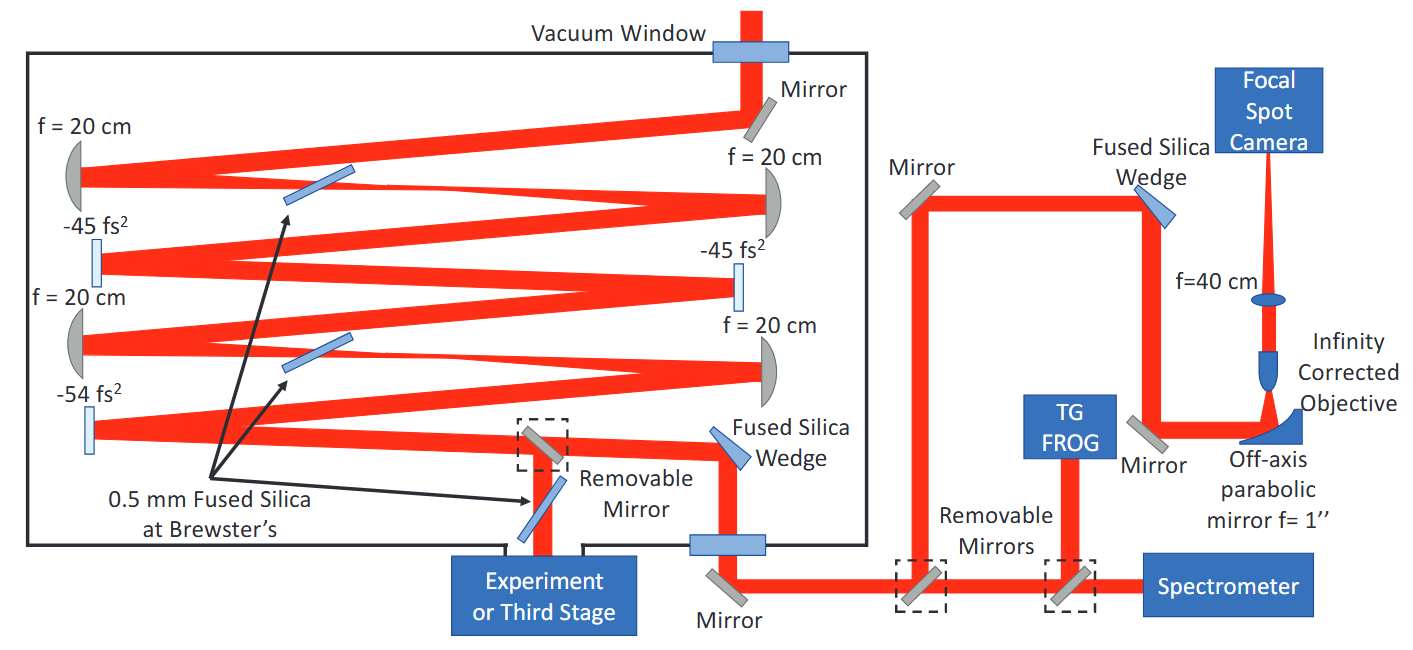
\includegraphics[width=0.7\textwidth]{p1.png}
    \caption{两级实验装置: 脉冲从顶部进入并被引导至由两个曲面镜组成的第一级反射望远镜. 光谱展宽发生在以布儒斯特角定向的 0.5 毫米熔融石英板内部. 每级中的准直曲面镜的位置都可以准直经历非线性透镜的加宽光束}\label{p1}
\end{figure}

输入: 市售单级钛蓝宝石再生放大器 (Spectra-Physics Solstice ACE) 

· 重复频率为千赫兹, 中心波长为 800 nm, P 偏振;

· 波前为高斯模式, M2 <1.25. 

· 通过在 -20 dB 水平下具有 70 nm 带宽的二次谐波发生频率分辨光选通 (SHG FROG) 测量, 初始脉冲持续时间为 36 fs. 压缩装置输入端传递的激光能量高达 6.9 毫焦耳, 相当于 180 GW 的最大峰值功率, 但大多数实验使用 0.95 mJ 来防止光学损伤. 

两级脉冲压缩方案

· 激光进入由两个曲面镜组成的反射式伽利略望远镜, 该望远镜通过焦点中继光束. 将一块熔融石英薄板放置在距焦点足够远的位置, 从而抑制材料的电离, 但又足够近, 从而存在非线性. 

· 在此介绍的所有实验中, 熔融石英上的强度约为 4 $\mathrm{TW\; cm^{-2}}$. 由于损伤阈值高、光学质量高且光学参数已知, 因此使用了熔融石英板;

· 可以通过将板放置在沿光轴的合适位置来调节熔融石英中的激光强度;

· 脉冲压缩装置安装在真空室内, 使激光能够通过焦点而不发生激光击穿. 

SPM介质: 500 $\mathrm{\mu m}$ 熔融石英板, 以布儒斯特角放置以最大限度减少反射损失, 将传播长度增加到 600 $\mathrm{\mu m}$. 

由于熔融石英板上的光束尺寸较小, 加宽光束的克尔透镜效应是不可忽略的, 这使得焦点移近望远镜的聚焦光学器件\cite{khazanovNonlinearCompressionHighpower2019}. 准直光学器件的放置是为了补偿这种非线性透镜, 输出准直、展宽的脉冲并减少望远镜的总长度. 未经过非线性透镜的剩余未展宽激光脉冲将以正发散度输出望远镜. 

脉冲在级间通过啁啾镜 (Newport 10Q20UF.40 和 Thorlabs UMC10-15FS) 压缩. 

· 能量吞吐量取决于所使用级数, 并受所用镜子反射率的限制. 例如, 两级系统的能量吞吐量为 $75 \pm 1\%$, 主要来自金属镜的使用. 

结果测量:

· 为在不引入额外非线性情况下暂时表征展宽光束, 通过在布鲁斯特角附近使用熔融石英楔子反射来降低光束强度. 

· 由于脉冲超连续谱性质, 通过将光束发送到瞬态光栅频率分辨光门控 (TG-FROG) 来对该脉冲进行时间表征. 光束可以从 TG-FROG 转移到 F/2 离轴抛物面 (OAP) 镜中以表征焦点. 

· 光场依赖性测量: 使用无限远校正平面消色差显微镜物镜和将焦点放大到数码相机上的成像镜头对焦点进行重新成像. 通过将介电带通滤波器 (Thorlabs FB650-40、Newport 10BPF10-700 和 Thorlabs FB800-10) 放置在焦斑成像光学器件的准直部分来测量远场的波长依赖性. 诊断与准直、多周期激光输出一致. 脉冲压缩器的加宽输出与诊断相一致, 无需改变任何成像条件. 在对展宽光束进行成像时, 未展宽光束的任何剩余部分都不会被正确准直, 因此会在 TG-FROG 和焦点表征设置中聚焦到不同的焦平面. 

· 展宽光谱分别通过测量光束空间平均值, 或者通过测量光束在屏幕上的漫散射, 或者通过将光束聚焦到余弦校正器和光纤光谱仪上. 两次测量产生相似结果且使用光谱仪经过 NIST 校准的卤钨灯进行校准. 如果可能, 取整个光束用于诊断和表征. 然而, 光束的发散未展宽部分 (优先存在于光束的外边缘) 被 TG-FROG 和第三级光谱测量中的硬孔径阻挡. 

\section{Result}

\subsection{Spectral broadening numerical modeling}

· PyNLO: 使用分步傅立叶法 (SSFM) 求解广义非线性薛定谔方程;\cite{hultFourthorderRungeKutta2007}

尽管在模拟中包含自陡峭和延迟拉曼响应与实验具有更好一致性, 但材料色散的影响最大. 材料色散根据熔融石英的四阶色散进行建模. 材料的厚度和熔融石英的位置与实验值相同. 在每个阶段之前, 都会考虑两个银镜 (Newport ER.2) 的反射损失. 由于目标以布儒斯特角定向以最大限度地减少反射损失, 因此熔融石英内的峰值强度有效降低了约 1.4. 模拟的初始脉冲与使用 SHG-FROG 进行的测量相匹配, 包括模拟空气和真空窗口中的非线性传播. 

模拟是一维的但与实验一致, 这是因为最高强度区域将产生最大带宽且在空间积分光谱中, 光谱极值来自该中心部分. 虽然二维模拟无疑有更好的一致性, 但通过实验观察到实验和模拟之间存在足够一致的相关性. 

尽管目标很薄, 但引入由材料色散引起的少量群延迟色散 (GDD) 将极大地改变SPM调制的输出光谱, 在不包括色散下, 2 级系统预测 FTL 脉冲持续时间比实验测量短 40\%. 在模拟和实验结果中都观察到不对称展宽, 这主要是由于许多激光系统固有的残余三阶相位造成的. 材料色散、自陡峭、延迟拉曼响应也导致光谱的不对称展宽. 

\subsection{Experimental compression}

作者通过数值模拟确定电介质板上强度以及啁啾反射镜所需色散补偿量. 

放置熔融石英板以产生预期的强度. 

\begin{figure}[h]
    \centering
    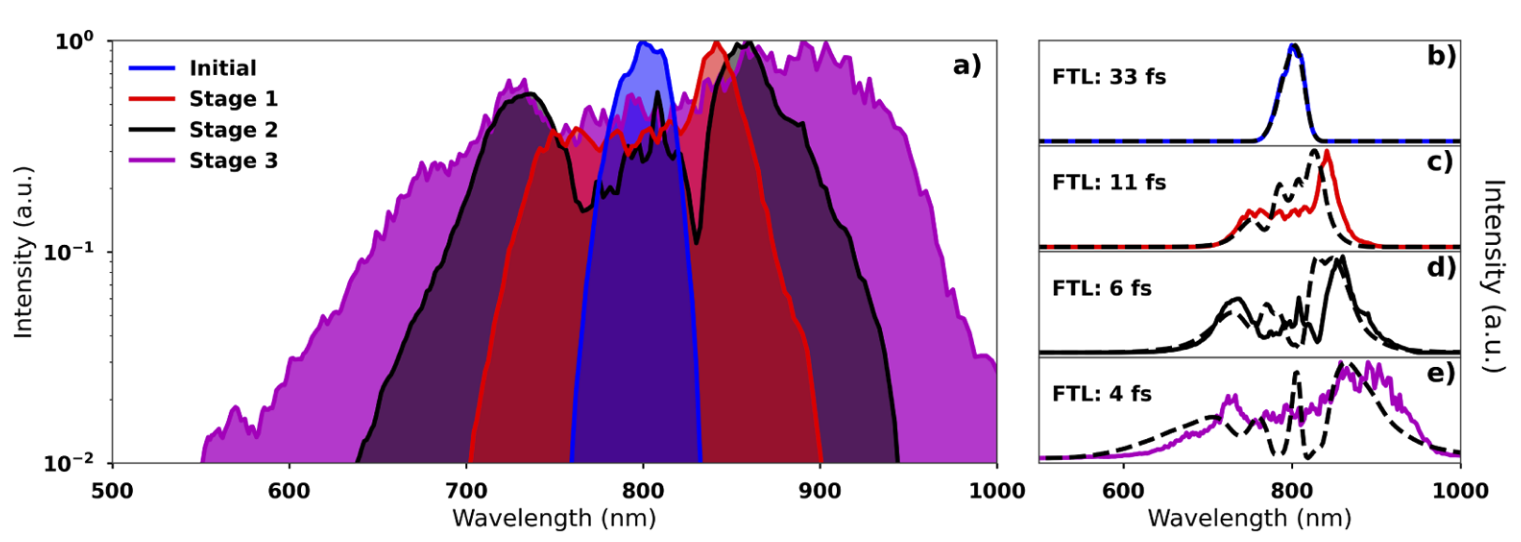
\includegraphics[width=0.7\textwidth]{p2.png}
    \caption{实验和模拟光谱: (a) 具有不同级数 (对数标度) 实验光谱测量. 初始脉冲 (蓝色) 的 -20 dB 宽度为 70 nm. 每级的输出带宽为: 第一级 (红色) 为 198 nm, 第二级 (黑色) 为 316 nm, 第三级 (品红色) 为 477 nm, 总展宽系数为 6.8. (b-e) 每个阶段实验输出光谱 (实线) 和线性模拟 (虚线), 列出了每个阶段对应变换极限. 仿真频谱给出变换极限最初为 35 fs, 1 级为 12 fs, 2 级为 6 fs, 3 级为 4 fs. }\label{p2}
\end{figure}

激光带宽几乎增加两倍至 198 nm, 中心波长保持为 800 nm, 对应于 12 fs 的 FTL 持续时间, 如图 \ref{p2} 所示. 

板上的光束直径, 激光系统最初输出为 12 mm, 板上约为 1 毫米. 

第一级后共使用 GDD -90 $\mathrm{fs^2}$ 压缩脉冲.

\subsection{Multi-staged compression}

多级压缩, 每级均由一对一的望远镜、0.5 mm 熔融石英板和啁啾镜组成. 

由于前一阶段时间压缩, 要增加每级的目标光束直径以保持恰当强度而不损坏熔融石英. 第二级和第三级的光束直径分别约为 1.7 mm 和 1.9 mm. 

第二级:

光谱展宽至 -20 dB 的 316 nm 宽度, 如图 \ref{p2}. 

色散通过啁啾镜的 -54 $\mathrm{fs^2}$ 和来自附加材料色散的 22 $\mathrm{fs^2}$ 色散的组合进行校正. 当消除传播到 FROG 的色散累积时, 测量到的检索脉冲持续时间为 7 fs, 接近 6 fs 的变换极限, 如图 \ref{p3} 所示. 

\begin{figure}[h]
    \centering
    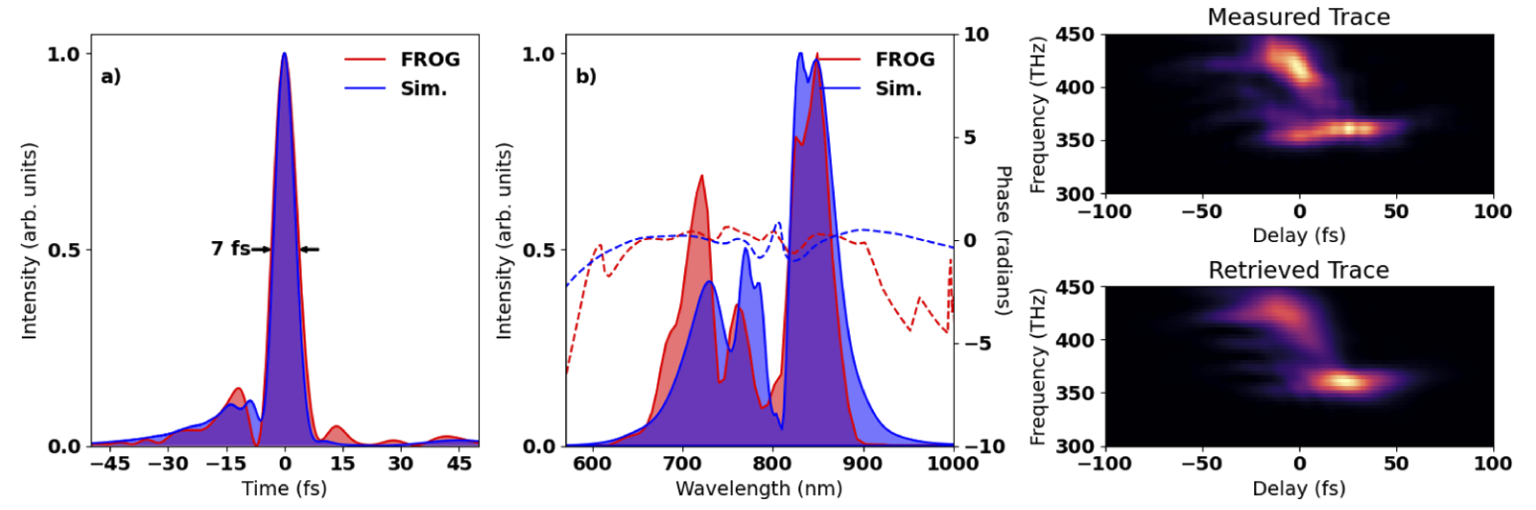
\includegraphics[width=0.9\textwidth]{p3.png}
    \caption{TG-FROG 重建: (a) TG-FROG 测量 (红色) 两级激光脉冲时间曲线, 脉冲持续时间为 7 fs (2-3 个周期) ；数值模拟 (蓝色) 显示相同的 7 fs 持续时间.  (b) 第二级输出频谱, 功率谱 (实线) 和频谱相位 (虚线) 重叠. 重建脉冲 (红色) 和数值模拟 (蓝色) 显示出良好的一致性.  (c-d) 实验测量和检索的 FROG 痕迹. }\label{p3}
\end{figure}

第三级:

· 光谱进一步展宽至 -20 dB, 477 nm 宽度, 对应 4 fs FTL 持续时间或亚两周期脉冲.

· 然而该频谱比可用啁啾镜带宽更宽, 因而无法压缩;

· 与之前阶段类似, 色散以 GVD 为主, 因此适合通过啁啾镜压缩. 模拟预测仍可通过 GDD 补偿压缩至 FTL. 

· 对于如此大的带宽, 前一级 GDD 的不完美补偿会对脉冲展宽产生重大影响. 对于第三级输入, 22 $\mathrm{fs^2}$ 的色散补偿误差会产生约 15\% 窄的频谱. 

两级增加能量: 两级压缩器输入能量增加至 6.9 mJ

· 相应光束直径增加至 24 mm, 以防第一阶段压缩后的光学损伤. 纵向调整熔融石英板, 以在熔融石英上保持与 0.95 mJ 情况大致相同的峰强度. 

· 6.9 mJ 下, 第二级展宽光谱几乎相同, FTL 脉冲持续时间为 8 fs, 

· 光谱差异源于传播到压缩器的额外非线性.  

· 6.9 mJ 光谱模拟预测 8.5 fs FTL. 

· 因为增加强度需要比可用啁啾镜更大的光束直径, 因而第二级输出无法压缩. 

\subsection{Focal spot characterization}

准直的、未展宽的光束用于对准焦点诊断并作为参考焦点. 当发送到焦点诊断时, 未展宽的光束聚焦到近衍射极限点, FWHM 为 $2.1 \times  1.8 \pm 0.1\; \mathrm{\mu m}$, 如图 \ref{p4} (a) 所示. 

\begin{figure}[h]
    \centering
    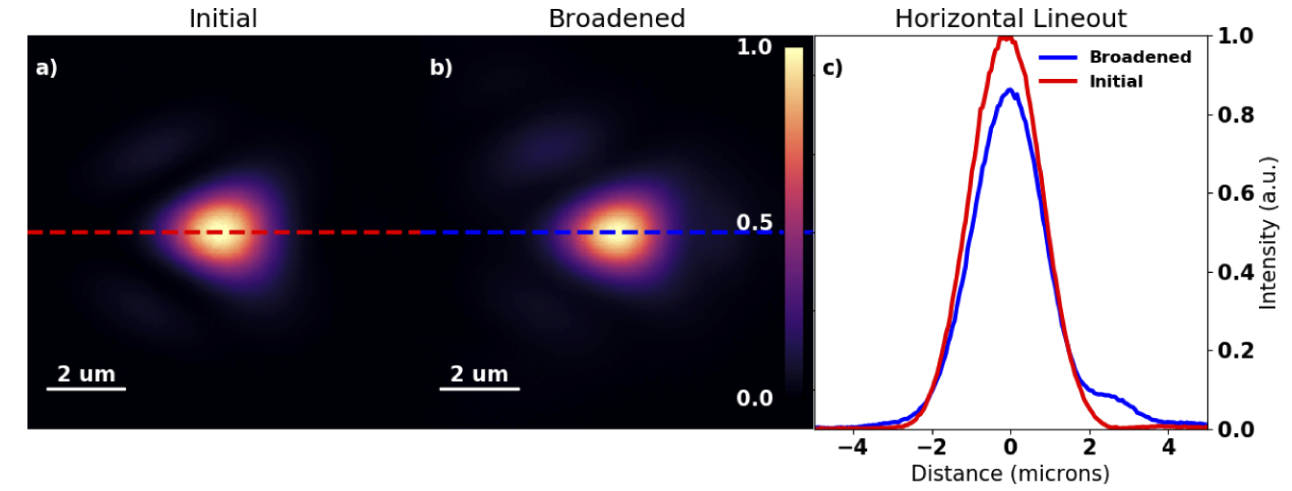
\includegraphics[width=0.7\textwidth]{p4.png}
    \caption{脉冲压缩前后焦点的相机图像: (a) 非展宽激光脉冲的焦点 (b) 展宽激光脉冲的焦点 (c) 焦点的水平轮廓线, 峰值计数和封闭能量下降了 15\%, 而整体形状基本保持不变, 仅在焦点上添加了少量额外的翼结构. }\label{p4}
\end{figure}

对于加宽的情况, 测量了接近相同的焦点, FWHM 为 $2.1 \times  1.7 \pm 0.1\; \mathrm{\mu m}$, 如图 \ref{p4} (b) 所示. 

· 焦点的形状基本上保持不变. 

· 出现轻微的翼结构, 导致 $1/e^2$ 焦径增加约 8\%. 

· 所有波长的光束质量基本相似, 所使用的每个带通滤波器的 $1/e^2$ 宽度平均在 10\% 以内. 

· 作者观察到每级的峰值注量仅下降约 7\%, 对于两个阶段, 峰值降低了 15\%, 如图 \ref{p4}(c) 所示. 同样, 通过在像平面上放置针孔的大面积光电二极管和热电堆功率计测量, 两级 $1/e^2$ 焦斑中包含的能量减少了约 14\%. 

\section{Discussion}

\subsection{光束特性}

在脉冲展宽的非线性方案中, 讨论光束特性时必须非常小心. 就展宽和脉冲持续时间而言, 光束轮廓可能存在一定程度的不均匀性. 在 TFC 的情况下, 

· 12 mm 光束以较低的 B 积分进入电介质, 会产生较窄的光谱, 但也会产生不易补偿的空间相位误差. 

· 在作者之前的激光系统中观察到, 当使用 TFC 几何形状时, 焦斑质量和强度存在显着损失\cite{khazanovNonlinearCompressionHighpower2019, farinellaDemonstrationThinFilm2019}. 这些损失似乎在本文系统中减轻. 光束聚焦性优于准直系统的机制无法使用相同模型来解释值得进一步研究. 一种可能解释是聚焦几何结构中的多级光谱展宽与电介质内部发生的非线性透镜之间存在相互作用. 

%--------------------  插入参考文献  --------------------%

\newpage

\clearpage           %%%  “目录”中显示的页码正确, 需要添加 \clearpage
\phantomsection      %%   “目录”中的链接能正确跳转, 需要添加 \phantomsection
\addcontentsline{toc}{section}{参考文献}   %向目录中添加条目, 以章的名义

\bibliography{ref}

\end{document}